\section{Results}

\begin{figure}
    \centering
    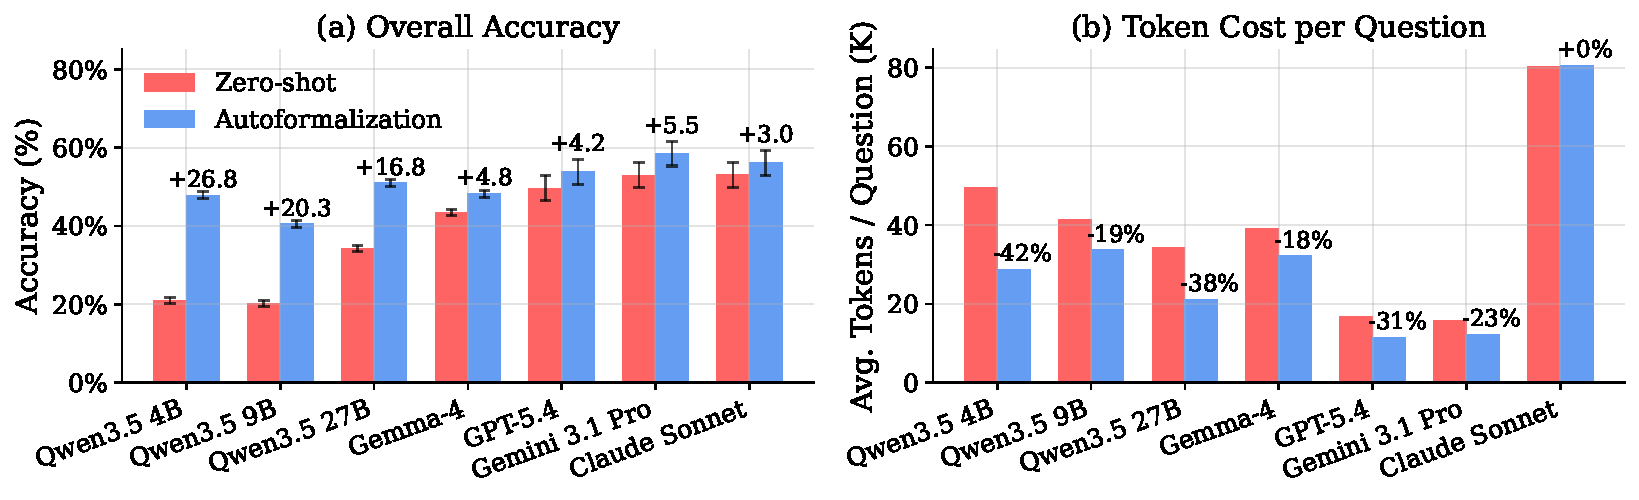
\includegraphics[width=1\linewidth]{figures/comparison_overall.pdf}
    \caption{Caption}
    \label{fig:placeholder}
\end{figure}

We organize our experimental evaluation around three questions:
(1) How difficult is clinical QA over real EHR databases for current LLMs?
(2) How does clinical autoformalization compare to alternative approaches?
(3) How well do autoformalized libraries generalize across guidelines, databases, and patient populations?
All autoformalization and inference experiments use \texttt{vllm}~\cite{kwon2023efficient} as the inference engine.
The autoformalization loop allows up to 100 exploration turns per concept with a context compression threshold of 25{,}000 tokens; the QA verification and inference agents are limited to 10 turns each.
A stratified subset of 100 patients per concept is used for verification during autoformalization, and evaluation is performed on the held-out 90\% test split (56{,}700 QA pairs).

%% ============================================================
%% 5.1 TASK DIFFICULTY: LLM PERFORMANCE BY DIFFICULTY LEVEL
%% ============================================================
\subsection{Task Difficulty}
\label{sec:task_difficulty}

To characterize the difficulty of \ours{} and establish the landscape for current LLMs, we evaluate a diverse set of models in a zero-shot code-generation setting. Each model is given the raw MIMIC-IV schema, a \texttt{query\_db} function, and a clinical question, and must iteratively generate executable code to retrieve and analyze information from the database. The model can then reason over execution outputs to produce an answer or continue refining its code, for up to 10 iterations. We select models spanning multiple families and scales to ensure broad coverage and to control for potential schema memorization from pretraining data, since MIMIC-IV is a widely studied dataset.

% ---- TABLE 1: LLM performance by difficulty level ----
\begin{table}[t]
\centering

\label{tab:llm_difficulty}
\resizebox{\linewidth}{!}{
\begin{tabular}{lcccccc}
\toprule
\multirow{2}{*}{Model} & \multicolumn{4}{c}{Accuracy by Difficulty Level} & \multirow{2}{*}{Overall} & \multirow{2}{*}{Tokens/Q} \\
\cmidrule(lr){2-5}
& Level 1 & Level 2 & Level 3+ & $\Delta$ (L1$\to$L3+) & & \\

\midrule
\multicolumn{7}{c}{\textbf{Frontier Models}} \\
\midrule

Claude-Sonnet-4.6  & 58.4 & 51.0 & 41.1 & -17.3 & 53.1 & 80308 \\
Gemini-Pro-3.1  & 58.0 & 54.1 & 37.2 & -20.8 & 53.0 & 15897* \\
GPT-5.4  & 55.1 & 47.8 & 36.7 & -18.4 & 49.6 & 16778 \\

\midrule
\multicolumn{7}{c}{\textbf{Open-Source Models}} \\
\midrule

Gemma4-31B        & 46.9 & 44.2 & 32.2 & -14.7 & 43.4 & 39243 \\
gpt-oss-120B      & 39.4 & 38.6 & 23.2 & -16.2 & 36.1 & \textbf{19576} \\
Kimi-K2.6         & 37.1 & 41.6 & 19.7 & -17.4 & 35.0 & 33017 \\
Qwen3.5-27B       & 36.5 & 38.6 & 21.6 & -14.9 & 34.2 & 34414 \\
Qwen3.5-9B        & 22.8 & 22.9 & 8.7 & -14.2 & 20.2 & 41378 \\
Qwen3.5-4B        & 25.4 & 20.9 & 8.6 & -16.8 & 21.0 & 49445 \\

\bottomrule
\end{tabular}
}
\caption{Zero-shot QA accuracy (\%) of LLMs on \ours{} by difficulty level. All models are given only the raw MIMIC-IV schema and a \texttt{query\_db} tool. Difficulty levels correspond to dependency-chain depth in the clinical concept graph (Section~3). Results are averaged across question types within each level.}
\end{table}

Table~\ref{tab:llm_difficulty} reports accuracy across all 63 concepts, grouped by difficulty level.
Several trends emerge.
First, even the strongest frontier models achieve only moderate accuracy overall, confirming that clinical QA over real EHR databases remains a challenging task that is far from saturated.
Second, performance degrades consistently from Level~1 to Level~3+ across all model families, with the drop (column $\Delta$) reflecting the compounding effect of multi-hop dependencies: answering a Sepsis-3 question requires correctly computing SOFA sub-scores, infection criteria, and antibiotic timing, each of which can independently fail.


%% ============================================================
%% 5.2 BASELINE COMPARISONS
%% ============================================================
\subsection{Comparison of Approaches}
\label{sec:baselines}

We compare several agentic setups to isolate the contribution of autoformalized code libraries.
All approaches use the same backbone LLM (\texttt{Qwen-3-4B}) at inference time.

\begin{enumerate}[label=\textbf{(\arabic*)},nosep,leftmargin=*]
    \item \textbf{Raw Schema + \texttt{query\_db}}: The LLM receives only the raw MIMIC-IV schema and a \texttt{query\_db} function. This is the zero-shot baseline from Section~\ref{sec:task_difficulty}.
    \item \textbf{RL Finetuning}: We finetune 3 different Qwen3 models of increasing scale (\texttt{Qwen3-4B}, \texttt{Qwen3-14B}, and \texttt{Qwen3-32B}) \cite{yang2025qwen3} using standard GRPO \cite{shao2024deepseekmath}. During training, the models receive only the MIMIC-IV schema and a \texttt{query\_db function}. We sample 5 training examples per concept for each model's training. Full training parameters are listed in the appendix section \ref{app:train_details}.
    \item \textbf{Clinical Autoformalization (Ours)}: The LLM is given the raw MIMIC-IV schema, a \texttt{query\_db} function, and the autoformalized function library $\mathcal{L}$ along with a retrieval tool to find and load relevant functions.
\end{enumerate}

% ---- TABLE 2: Baseline comparison ----
\begin{table}[t]
\centering
\caption{Comparison of QA approaches across all 63 concepts on the held-out test set. Accuracy is macro-averaged across concepts. Token usage and time are reported per question at inference. \textcolor{red}{[TODO: Fill in all cells. Add a row for ``Human Expert'' if available. Consider adding F1 for binary questions in addition to accuracy.]}}
\label{tab:baselines}
\resizebox{\linewidth}{!}{
\begin{tabular}{lcccccc}
\toprule
\multirow{2}{*}{Method} & \multicolumn{3}{c}{Accuracy by Level} & \multirow{2}{*}{Overall Acc.} & \multirow{2}{*}{Tokens/Q} & \multirow{2}{*}{Time/Q (s)} \\
\cmidrule(lr){2-4}
& Level 1 & Level 2 & Level 3+ & & & \\
\midrule
(1) Raw Schema + \texttt{query\_db}         & 44.9 & 32.8 & 26.3 & 38.1 & 30479 & 3.1 \\
(2) GRPO Finetuning                    & -- & -- & -- & -- & -- & -- \\
(3) Autoformalization (Ours)                 & 51,2 & 41.5 & 34.1 & 45.3 & 23569 & 2.5 \\
\midrule
\multicolumn{7}{c}{\textbf{Frontier Models}} \\
\midrule
\bottomrule
\end{tabular}
}
\end{table}

Table~\ref{tab:baselines} summarizes the results.
Approach~(1) confirms that raw schema access alone is insufficient for reliable clinical QA, particularly at higher difficulty levels where the model must independently discover and correctly combine multiple derived quantities.
Approach~(2), finetuning, is moderaly better

Approach~(3), our autoformalization pipeline, achieves accuracy competitive with the derived-schema oracle while operating entirely on the raw schema, demonstrating that the offline verification loop produces functions of comparable quality to hand-curated SQL transformations.
Crucially, autoformalization reduces per-query token usage by \textcolor{red}{X\%} compared to (1), since the agent calls compact pre-verified functions rather than re-exploring the schema from scratch for each question.












\begin{table}[t]
\centering

\label{tab:baselines}
\resizebox{\linewidth}{!}{
\begin{tabular}{lcccccc}
\toprule

 \textbf{Model} & Level 1 & Level 2 & Level 3+ & \multirow{2}{*}{Overall Acc.} & \multirow{2}{*}{Tokens/Q} & \multirow{2}{*}{Time/Q (s)} \\
\midrule
(1) Raw Schema + \texttt{query\_db}         & 44.9 & 32.8 & 26.3 & 38.1 & 30479 & 3.1 \\
(2) GRPO Finetuning                    & -- & -- & -- & -- & -- & -- \\
(3) Autoformalization (Ours)                 & 51,2 & 41.5 & 34.1 & 45.3 & 23569 & 2.5 \\
\midrule
\multicolumn{7}{c}{\textbf{Frontier Models}} \\
\midrule
\bottomrule
\end{tabular}
}
\caption{Comparison of QA approaches across all 63 concepts on the held-out test set. Accuracy is macro-averaged across concepts. Token usage and time are reported per question at inference. \textcolor{red}{[TODO: Fill in all cells. Add a row for ``Human Expert'' if available. Consider adding F1 for binary questions in addition to accuracy.]}}
\end{table}

\begin{tabular}{lcccccccc}
\toprule
Model & Acc$\uparrow$ & Prio$\uparrow$ & Alert F1$\uparrow$ & 
$\Delta t_{\text{alert}}$ (h)$\downarrow$ & Miss$\downarrow$ & 
Tokens$\downarrow$ & Runtime (s)$\downarrow$ & Tool Calls \\
\midrule
Ours & 84.6 & 76.9 & 0.0 & 0.0 & 0 & 75k & 304 & 30 \\
\bottomrule
\end{tabular}